%!TEX program = xelatex
% 完整编译: xelatex -> biber/bibtex -> xelatex -> xelatex
\documentclass[lang=cn,a4paper]{elegantpaper}

\title{众筹项目成功率影响因素的实证分析及成功率预测——以Makuake为例}
\author{李峥昊}
\institute{{西安交通大学\quad 大数据001}}

\date{\zhtoday}


% 本文档命令
\usepackage{array}
\newcommand{\ccr}[1]{\makecell{{\color{#1}\rule{1cm}{1cm}}}}
\addbibresource[location=local]{reference.bib} % 参考文献,不要删除

\begin{document}

\maketitle

\begin{abstract}
\quad\quad 本文从Makuake众筹网站中获取了全部29658条众筹数据,构建了Makuake众筹数据集,并基于Makuake数据集分析了众筹项目成功率的影响因素。用机器学习和深度学习中的多种方法构建了众筹项目成功率预测模型,并训练了一个文本分类模型以帮助用户自动填写项目类别。实验结果表明,目标金额对于众筹成功率有着较强的负面影响,众筹选项中的金额设置对于成功率有多种影响。摘要长度、目标金额、活动数量等在预测过程中有着重要影响。文本特征对于准确率的提升较为有限。
\keywords{众筹,成功率,预测模型,文本分类,Makuake}
\end{abstract}


\section{介绍}
众筹(Crowdfunding)是近年来在网络上流行的一种融资方式,它为那些希望获得资金以创办或发展个人或团体项目的人提供了一种新的选择。众筹项目通常通过众筹平台发布在互联网上,以吸引潜在的支持者对项目进行资助。支持者通常会获得项目的一些奖励,这些奖励的数量和种类取决于支持者所提供的金额。

众筹模式有很多种,包括奖励型众筹、股权型众筹、债权型众筹和捐赠型众筹。奖励型众筹是最常见的模式。奖励型众筹为投资者提供非货币奖励,如资助项目的折扣\footnote{资助项目的折扣:可以以“早鸟价”或“尝鲜价”购买商品},资助项目的预购\footnote{资助项目的预购:如手办、周边等商品的发售往往预购-制作-售卖的形式,除了预购,只有少量商品公开售卖},或其它象征赞赏的奖励\footnote{象征赞赏的奖励:非卖品,如「在这世界的角落」中的奖励的明信片;权利,如可以参加“生产支持者会议”}~\citep{10.1007/978-3-030-29035-1_53}。奖励型众筹一般来说有两种模式,“All or Nothing”和“All in”(Makuake),“All or Nothing”和“Keep it All”(Kickstarter)。

众筹在网络上的流行主要得益于互联网的普及和社交媒体的发展。这些平台为项目发起者提供了一种方便的方式来宣传自己的项目,同时也为支持者提供了一种方便的方式来了解并支持感兴趣的项目。

然而,众筹并不是没有风险的。一些项目发起者可能会许诺不能兑现的奖励,或者甚至是故意欺骗支持者。为了减少风险,支持者可以选择只支持那些具有较强信誉的众筹平台。此外,支持者还应该加强对项目的了解,确保自己对项目有充分的了解,并对自己的支持进行适当的风险评估。

众筹项目的成功率受到许多因素的影响,总体上可以分为三类:众筹项目本身的特点,网络以及可理解性。其中众筹项目本身特点包括众筹目标金额,最低投资额,项目持续时间和提供的财务信息等~\citep{LUKKARINEN201626}。一般来讲,对于奖励型众筹,众筹目标金额对于成功率有负面影响~\citep{ZHENG2014488,https://doi.org/10.1111/fima.12262}。最低投资金额对成功率没有显著影响~\citep{agrawal2014some}。项目持续时间在欧美对于项目的成功率有负面影响,持续时间较长给了投资者较长的思考时间,以至于投资者们有可能忘记这件事~\citep{MOLLICK20141,H2014Crowdfunding},但是在中国,持续时间对于项目成功率有正面影响~\citep{ZHENG2014488}。在奖励型众筹中,社交网络的规模与项目的成功率有着显著的正相关关系\citep{etter2013launch}。在可理解性方面,产品类项目相较于服务类项目有更高的成功率,因为消费者们更愿意看到有形的结果\citep{belleflamme2013individual}。项目更容易被投资者理解对于众筹成功率有着正面影响\citep{H2014Crowdfunding}。




\section{数据选取说明}
\subsection{Makuake简介}
\begin{figure}[!htbp]
  \centering
  \includegraphics[width=4in]{makuake.png}
  \caption{Makuake众筹平台}
  \label{fig:Makuake}
\end{figure}
\href{https://www.makuake.com}{Makuake}是日本的一家众筹平台。于2013年8月作为\emph{CyberAgent(日本最大的网络广告代理商)}的新事业部成立。自2017年glafit电助力自行车以1亿日元以上的筹集金额破了日本国内众筹记录之后,逐渐成为为日本最大的众筹平台。平台众筹项目囊括了日常用品,时尚单品,餐饮店,日本酒,电影等各类行业的各种产品。代表作有动画\href{https://www.makuake.com/project/konosekai/}{「在这世界的角落」},日本酒\href{https://www.makuake.com/project/fuyuhitoe/}{「雪どけ酒」},耳机\href{https://www.makuake.com/project/vie-fit/}{「VIE FIT」},电助力自行车\href{https://www.makuake.com/project/glafit/}{「glafit」}等等(如图\ref{fig:makuake project}所示)。
\begin{figure}[!htbp]
  \centering
  \captionsetup[subfigure]{labelformat=empty}
  \subfigure[在这世界的角落]{\includegraphics[height=1.5in]{image/この世界の片隅に.png}}
  \subfigure[雪どけ酒]{\includegraphics[height=1.5in]{image/雪どけ酒.jpg}}
  \subfigure[VIE FIT]{\includegraphics[height=1.5in]{image/VIE FIT.png}}
  \subfigure[glafit]{\includegraphics[height=1.5in]{image/glafit.jpg}}
  \caption{Makuake代表项目}
  \label{fig:makuake project}
\end{figure}

\subsection{网页信息说明}
Makuake的项目界面主要分为3个页面,主界面,活动界面以及应援界面。
\begin{figure}[!htbp]
  \centering
  \subfigure[页首]{\includegraphics[height=2.4in]{image/makuake project1.png}}
  \hspace{0 pt}
  \subfigure[介绍]{\includegraphics[height=2.4in]{image/makuake project4.png}}
  \caption{主界面}
  \label{fig:main project}
\end{figure}

主界面的页首(如图\ref{fig:main project}所示)包含该项目的一些基本信息,如标题、筹集金额、目标金额,facebook点赞数量等等。

主页面的左侧部分包含介绍的摘要和主体部分,右侧包含项目的类型和可以选择的若干种支援方式。项目类型分为All in和All or nothing。All in表示不论筹集了多少钱,项目发起者都会收到这笔钱,并且要履行对应的服务,All or nothing 如果没有达到目标金额,则筹集金额全数返还。若干种支援方式,即项目发起人往往会在这里设置若干种不同价位不同组合的选项——以电影「在这世界的角落」为例,如果支付2160日元,则可以收到不定期的制作进度、动画草图的邮件,以及一张明信片;如果支付5400日元,则在前一档的基础上,可以参加导演举行的“生产支持者会议”。

\begin{figure}[!htbp]
  \centering
  \includegraphics[width=3in]{image/makuake project2.png}
  \caption{活动页面}
  \label{fig:project2}
\end{figure}

活动页面(如图\ref{fig:project2}所示),包含项目的进度信息。

\begin{figure}[!htbp]
  \centering
  \includegraphics[width=3in]{image/makuake project3.png}
  \caption{应援页面}
  \label{fig:project3}
\end{figure}

应援界面(如图\ref{fig:project3}所示)是支持者对于该项目的应援或是评论,只有参与了众筹的用户可以评论,可以多次评论。

\subsection{数据说明}
本次实验数据从5个url【项目主页,investment(项目主页的补充信息),facebook点赞数,活动,评论】中获取了共计31个字段的信息,以半结构化数据的形式存储在MongoDB中,每个字段的数据类型和含义如表\ref{tbl:变量说明}所示。

\begin{table*}
\centering
\caption{变量说明}
\begin{tabular}{ccc}
\toprule
字段&数据类型&含义\\
\midrule
id\_ &int &      每个项目的专属id       \\
 collected\_money  &str &         已筹集金额          \\
collected\_supporter&str &       支持者人数          \\
 expiration\_date  &int &      结束时间的时间戳       \\
     percent      &int &   筹集金额与目标金额之比    \\
    image\_url     &str &         缩略图地址          \\
      title       &str &          项目标题           \\
       url        &str &         详情页网址          \\
      is\_new      &bool&        是否是新项目         \\
 is\_store\_opening &bool&      是否可在商店购买       \\
 has\_target\_money &bool&       是否有目标金额        \\
  has\_expiration  &bool&       是否有截止日期        \\
is\_accepting\_support &bool&     是否接受支持         \\
hide\_collected\_money &bool&    是否隐藏筹集金额       \\
  returns      & array&             --              \\
is\_new\_store\_opening& bool&是否可以在Makuake STORE上购买\\
   summary\_text   &text&        摘要部分文字         \\
    main\_text     &text&      主要介绍部分文字       \\
  target\_amount   &str &          目标金额           \\
    thumb\_ups     &str &       facebook点赞数        \\
   activity   & Object&      所有活动的相关信息      \\
     start\_at     &str &          开始日期           \\
      end\_at      &str &          截止日期           \\
    curr\_time     &str &          当前日期           \\
      tag        & array&          所有标签           \\
     category     &str &            类别             \\
     location     &str &          项目位置           \\
  type\_       &str & 项目类型(all in/all or nothing) \\
   choice\_list  & array&        购买选项详情         \\
  img\_left\_href  & array&    介绍页面的图片url      \\
   comment\_list  & array&          所有评论           \\
\bottomrule
\end{tabular}
\label{tbl:变量说明}

\end{table*}



\section{数据抽取}
原始数据为通过爬虫获取的非结构化数据,需要通过数据抽取将非结构化数据转换为可以直接使用的、剔除无用信息的结构化数据。在数据抽取中对原始数据进行了以下操作:
\subsection{数据类型转换}
\begin{enumerate}
\item 将字符串格式保存的数值类型数据转换为整型或浮点型
\item 将字符串类型保存的日期类型数据转换为时间戳的形式\footnote{Unix时间戳(Unix timestamp)是一种时间表示方式,定义为从格林威治时间1970年1月1日起至现在的总秒数}
\item 将布尔类型的数据转换为0-1变量
\end{enumerate}

\subsection{数据特征抽取}
\begin{enumerate}
\item 对于文本信息(title, summary text, main text),获取文本长度,并作为新的变量
\item 对于活动信息(activity),获取活动数目,并作为新的变量
\item 对于评论信息(comment\_list),获取评论数目,并作为新的变量
\item 对于图片信息(img\_left\_href),获取图片数目,并作为新的变量
\item 对于标签信息(tag),获取标签数目,并作为新的变量
\end{enumerate}

\subsection{生成新的特征}
\begin{enumerate}
\item is\_end:通过计算\textbf{数据获取时间}与\textbf{项目结束时间}之差判断项目是否已结束
\item remain\_time:如果项目已结束,则剩余时间为0,否则剩余时间为\textbf{项目结束时间}-\textbf{数据获取时间}
\item conditon:通过percent和is\_end判断项目状态:成功、失败、进行中
\item duration:项目持续时间
\item min\_price, max\_price, avg\_price:\textbf{购买选项}中价格的最小值、最大值和均值
\end{enumerate}



\section{数据探索性分析}
\subsection{数据描述性统计}
描述性统计是一种汇总统计,用于定量描述或总结信息集合的特征。通过df.describe()生成的描述性统计如表\ref{tbl:描述性数据统计}所示。

\begin{table*}[!htbp]
\centering
\caption{描述性数据统计}
  \begin{tabular}{ccccccccc}
  \toprule
  字段&count&mean &std &min &25\% &50\% &75\% &max\\
  \midrule
  id\_&29658&15297.69&8723.78&1&7724.25&15256.5&22853.75&30415\\
  collected\_money&29658&2401211.73&9344913.74&0&280595&724550&1980617.5&623650600\\
  collected\_supporter&29658&217.8&574.41&0&28&79&203&29231\\
  percent&29658&952.37&2600.46&0&108&290&825&104195\\
  title\_length&29658&36.98&4.19&5&36&39&40&59\\
  is\_new&29658&0&0.07&0&0&0&0&1\\
  is\_store\_opening&29658&0.13&0.34&0&0&0&0&1\\
  has\_target\_money&29658&1&0.02&0&1&1&1&1\\
  has\_expiration&29658&1&0.01&0&1&1&1&1\\
  is\_accepting\_support&29658&0.03&0.18&0&0&0&0&1\\
  hide\_collected\_money&29658&0&0.01&0&0&0&0&1\\
  is\_new\_store\_opening&29658&0.13&0.34&0&0&0&0&1\\
  summary\_text\_length&29658&89.24&46.94&0&75&105.5&124&432\\
  main\_text\_length&29658&3556.49&1723.84&4&2370&3267&4408&20649\\
  target\_amount&29658&464409.5&1270125.98&0&100000&300000&500000&79600000\\
  thumb\_ups&29658&240.92&539.87&0&5&52&235&9427\\
  activity\_num&29658&9.59&9.9&0&3&7&13&228\\
  comment\_num&29658&27.82&74.34&0&4&11&28&5156\\
  start\_at&29658&1.6E+09&6.06E+07&1.38E+09&1.57E+09&1.62E+09&1.64E+09&1.67E+09\\
  end\_at&29658&1.6E+09&6.02E+07&1.38E+09&1.58E+09&1.62E+09&1.65E+09&1.68E+09\\
  curr\_time&29658&1.67E+09&135158&1.67E+09&1.67E+09&1.67E+09&1.67E+09&1.67E+09\\
  is\_end&29658&0.97&0.17&0&1&1&1&1\\
  remain\_time&29658&75169.13&503535.09&0&0&0&0&7268658\\
  duration&29658&4.00E+06&2.36E+06&-2.60E+08&2.71E+06&3.74E+06&5.12E+06&2.50E+07\\
  tag\_num&29658&8.51&1.21&4&9&9&9&12\\
  choice\_num&29658&8.03&4.79&1&5&7&10&106\\
  min\_price&29658&9378.47&22317.05&100&2680&4780&9900&1500000\\
  max\_price&29658&86633.05&321840.8&500&12411.5&24800&55200&10000000\\
  avg\_price&29658&27721.26&61186.59&500&7535.42&13600&26555.56&2694428.57\\
  img\_num&29658&29.88&17.13&0&17&27&39&274\\
  \bottomrule
  \end{tabular}
\label{tbl:描述性数据统计}
\end{table*}

从中我们可以看到,collected\_money,collected\_supporter,percent,target\_amount,thumb\_ups,comment\_num,min\_price,max\_price,avg\_price的分布都有较为严重的右偏。

几乎所有的商品都不是新商品(is\_new),几乎所有商品都有目标金额(target\_money)和截止日期(expiration),几乎所有的商品都没有隐藏筹集金额(collected\_money)。另外,有13\%的商品开放商店,有3\%的商品接受支持。




\subsection{数据可视化}
\subsubsection*{核密度图:不同状态项目的变量分布差异}
通过核密度图,我们可以更清晰地看到数据的分布。从图\ref{fig:displot}中可以看出,除了描述性统计中提到的几个极度右偏的数据,choice\_num,thumb\_ups,activity\_num也有较为严重的右偏现象。此外,start\_at,end\_at,有左偏的现象,表明随着时间发展,网站的项目和活跃用户越来越多。summary\_text出现双峰分布,有大量的数据集中在0和100附近,tag\_num有大量数据集中在9个和8个。
\begin{figure}[!htbp]
  \centering
  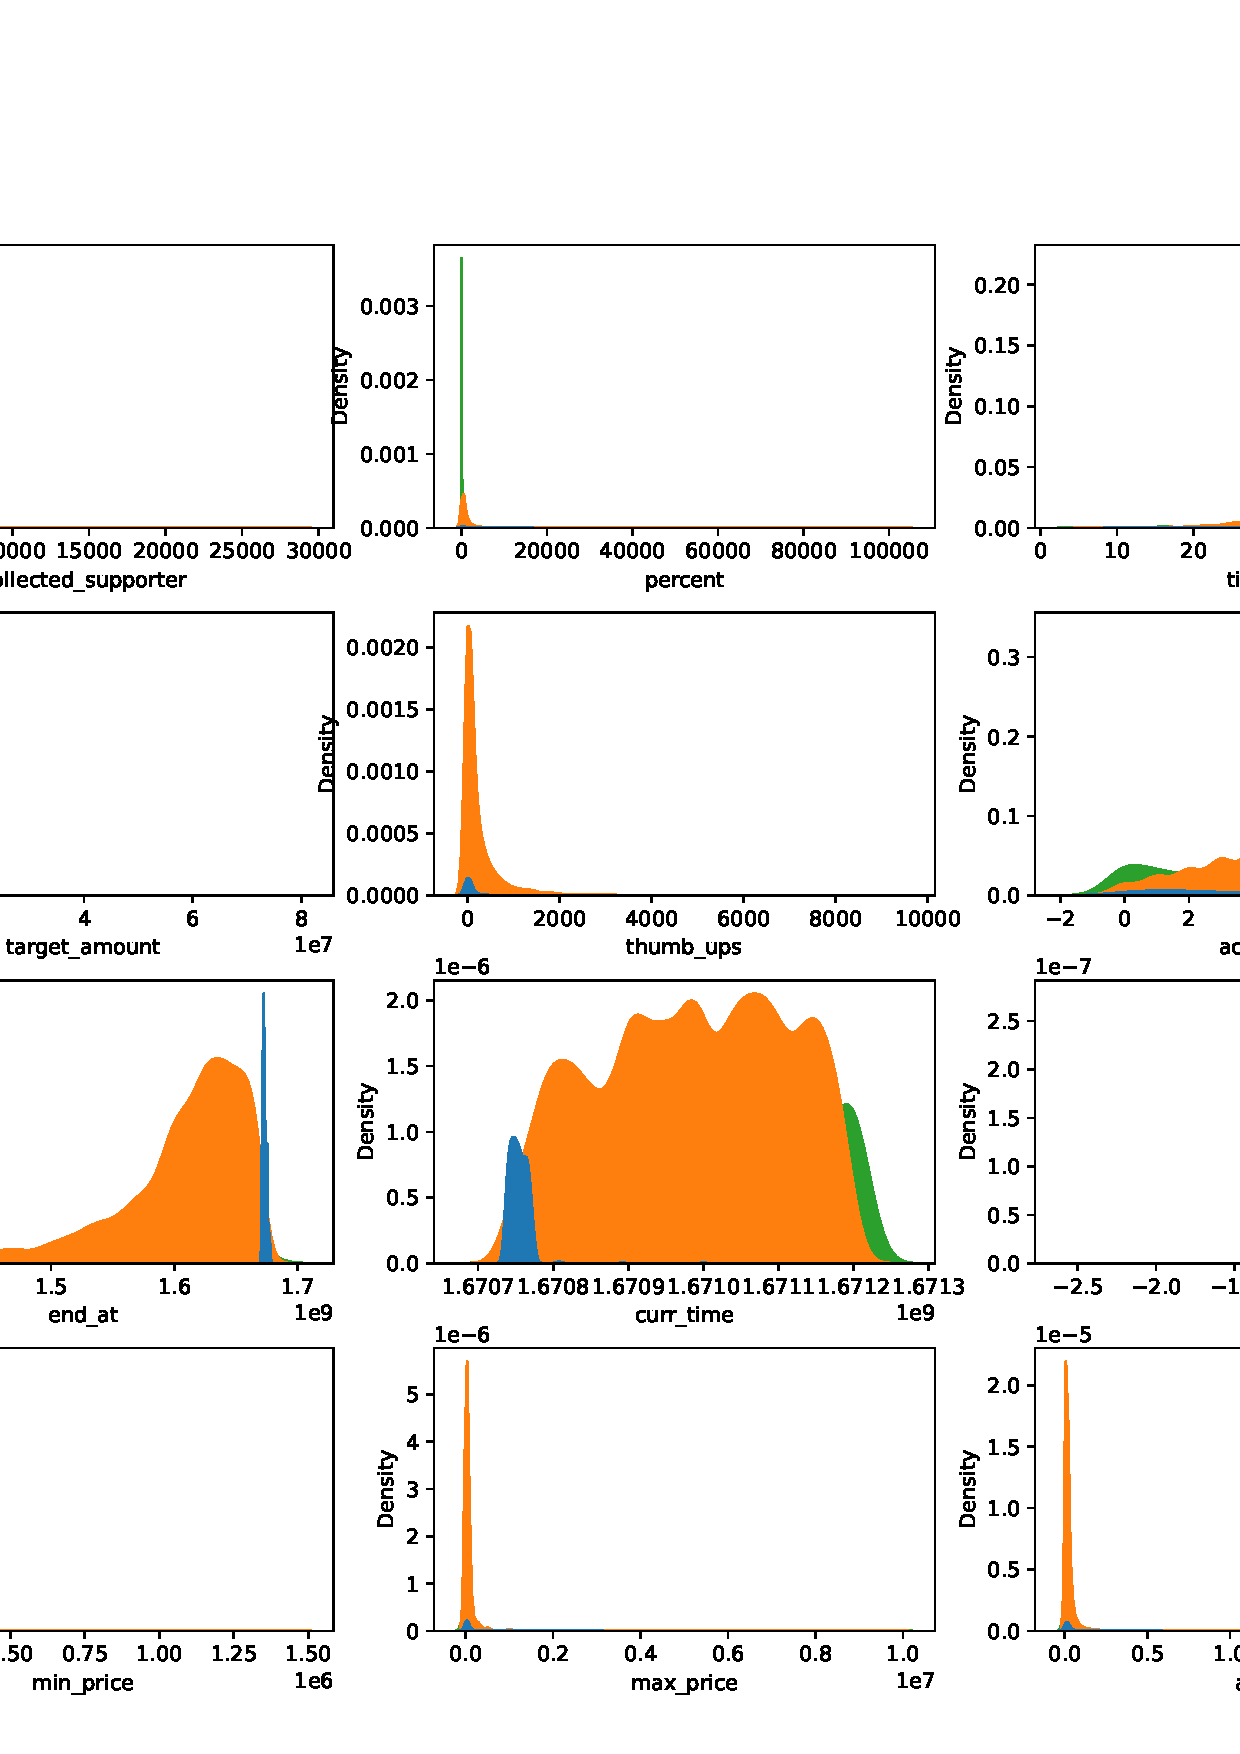
\includegraphics[width=\linewidth]{image/hist.pdf}
  \caption{不同状态项目的分布差异}
  \label{fig:displot}
\end{figure}

\subsubsection*{箱线图:不同状态项目的变量分布差异}
\begin{figure}[!htbp]
  \centering
  \includegraphics[width=\linewidth]{image/box.pdf}
  \caption{不同状态项目的均值及分布差异}
  \label{fig:boxenplot}
\end{figure}

随后通过箱线图(如图\ref{fig:boxenplot}所示)来更详细地观察不同状态的项目的均值和分布的差异。在箱线图中,对于前文提到的右偏数据进行了对数处理,以减少数据的偏态。

通过箱线图,可以发现,相较于失败的项目而言,成功的项目在均值和分布意义上都具有更长的标题,更长的摘要,更长的介绍,更多的活动,更多的标签,更高的最低价格,更多的选择以及更多的图片。具有更低的目标金额,更短的持续时间,更低的最低价格以及更低的平均价格。



\subsubsection*{条形图:类别变量中不同状态项目所占的比例}
通过条形图,可以展示成功、失败、进行中的比例与不同类别变量的关系,如图\ref{fig:label}所示。
从中我们可以看到技术类(テクノロジー),化妆品美容类(コスメ$\cdot$ビューティー),产品类(プロダクト),时尚类(ファッション),食物类(フード)以及餐厅酒吧类(レストラン$\cdot$バー)有较高的成功率。在爱媛、秋田、富山等地发布的项目有较高的成功率。 all in 类型的的项目有较高的成功率。另外,由于只有众筹成功的项目可以在makuake中进行贩卖,所以“贩卖中”的成功率为1。
\begin{figure}[!htbp]
  \centering
  \includegraphics[width=\linewidth]{image/label.pdf}
  \caption{类别变量中不同状态项目所占的比例}
  \label{fig:label}
\end{figure}


\subsubsection*{相关系数矩阵}
相关系数矩阵如图\ref{fig:corr}所示。显然,筹集金额与目标金额值比(percent)与筹集金额,支持者人数,点赞数,评论数,标题长度,图片数量,活动数量正相关,与目标金额负相关。
\begin{figure}[!htbp]
  \centering
  \includegraphics[width=\linewidth]{image/heatmap.pdf}
  \caption{相关系数矩阵}
  \label{fig:corr}
\end{figure}


\section{模型一:利用OLS分析众筹项目完成度的影响因素}
普通最小二乘法(OLS)是一种根据被解释变量的所有观测值与估计值之差的平方和最小的原则求得参数估计量的方法。最小二满足弗里施$\cdot$沃定理(Frisch Waugh theorem),即解释变量$x_1$的估计系数代表了$x_1$剔除了其它解释变量相关的部分对被解释变量$y$的影响。因此可以单独衡量某个解释变量对于被解释变量的影响。

项目完成度定义为筹款金额与目标金额之比,即:
\begin{align*}
\text{percent} = \frac{\text{collected\_money}}{\text{target\_amount}}
\end{align*}

\subsection{变量选取}
由于在已结束项目中,is\_end均为1,remain\_time均为0,故剔除这is\_end和remain\_time两个变量。由于duration = end\_at - start\_at,为线性关系,故剔除end\_at。最后将tag,category,type\_三个类别变量转换为哑变量。collected\_money,target\_amount,activity\_num,min\_price,max\_price,avg\_price 6个变量进行了对数处理。最终得到93个变量。由于研究的是完成度的影响因素,因此并未剔除筹集金额、点赞数、支持者人数等在项目发布时并未得知的变量。
\subsection{回归结果}
回归结果如表\ref{tbl:回归结果}所示。
\begin{table*}[!htbp]
\centering
\caption{回归结果}
  \begin{tabular}{cccccc}
  \toprule
  变量&coef&变量&coef&变量&coef\\
  \midrule
  const&\textcolor{red}{-68.9091***}&ファッション&\textcolor{red}{-6.7353**}&島根&0.4984\\
 collected\_money&\textcolor{red}{1.8981***}&フード&\textcolor{red}{-4.5698*}&広島&\textcolor{red}{-2.8166**}\\
  collected\_supporter&\textcolor{red}{0.0283***}&プロダクト&\textcolor{red}{-4.6163*}&徳島&-2.5706\\
  thumb\_ups&\textcolor{red}{0.002***}&レストラン・バー&-4.4356&愛媛&-0.4509\\
  comment\_num&\textcolor{red}{-0.0299***}&世界一周&-3.2019&愛知&-0.3965\\
  title\_length&0.0289&出版・ジャーナリズム&-5.0591&新潟&-0.2655\\
  is\_store\_opening&\textcolor{red}{-1.4346**}&地域活性化&-2.6483&東京&\textcolor{red}{0.7819*}\\
  has\_target\_money&\textcolor{red}{85.1172***}&教育&-3.4429&栃木&0.55\\
  has\_expiration&17.3102&映画・映像&-1.4503&沖縄&-0.3018\\
  is\_accepting\_support&-1.9068&演劇・パフォーマンス&-1.7738&海外&\textcolor{red}{1.1501**}\\
  hide\_collected\_money&\textcolor{red}{50.2516***}&社会貢献&-2.6114&滋賀&1.9262\\
  is\_new\_store\_opening&-4.3593&音楽&-3.0526&熊本&-0.3406\\
  summary\_text\_length&-0.0035&京都&0.074&石川&\textcolor{red}{-2.863*}\\
  main\_text\_length&3.25E-05&佐賀&-1.2703&神奈川&0.2407\\
  target\_amount&\textcolor{red}{-8.0092***}&兵庫&-0.3067&福井&-0.9019\\
  activity\_num&-0.2013&北海道&-0.8359&福岡&0.9936\\
  start\_at&3.02E-09&千葉&-0.1602&福島&3.174\\
  duration&\textcolor{red}{5.62E-07***}&和歌山&\textcolor{red}{-3.1825**}&秋田&-2.0288\\
  tag\_num&\textcolor{red}{-0.7564***}&埼玉&\textcolor{red}{1.5824*}&群馬&-1.9678\\
  choice\_num&\textcolor{red}{0.1152***}&大分&-1.103&茨城&-3.2234\\
  min\_price&\textcolor{red}{0.417**}&大阪&-0.5965&長崎&-2.507\\
  max\_price&\textcolor{red}{-4.2687***}&奈良&-1.3047&長野&-1.1228\\
  avg\_price&\textcolor{red}{8.8882***}&宮城&-0.7251&青森&-0.1758\\
  img\_num&\textcolor{red}{0.0695***}&宮崎&-2.8677&静岡&-0.5138\\
  アニメ・マンガ&\textcolor{red}{-6.245**}&富山&-1.9041&香川&-2.3568\\
  アート・写真&-3.2746&山口&-0.8265&高知&-1.1573\\
  ゲーム&-4.7568&山形&-0.4824&鳥取&0.5406\\
  コスメ・ビューティー&-3.9703&山梨&-1.1832&鹿児島&-0.2419\\
  スタートアップ&-3.6069&岐阜&-1.0377&type\_\_All or nothing&\textcolor{red}{2.2701}\\
  スポーツ&-3.6863&岡山&-1.1239&type\_\_others&50.2516***\\
  テクノロジー&0.3499&岩手&-0.0118&type\_\_販売中&5.8977\\

  \bottomrule
  \end{tabular}
\label{tbl:回归结果}
\end{table*}
从中可以看到,筹集金额(collected\_money)、支持者人数(collected\_suporter)、评论数(comment\_num)、是否有目标金额(has\_target\_money)、是否隐藏已筹集金额(hide\_collected\_money)、目标金额(target\_amount)、持续时间(duration)、标签数量(tag\_num)、可选择支持方式的数量(choice\_num)、众筹最大金额(max\_price)、众筹平均金额(avg\_price)、众筹类型All or Nothing(type\_\_All or Nothing)对项目完成度有着显著影响。

其中,筹集金额、支持人数、点赞数、持续时间、选择数量、平均价格、图片数量、筹集类型中的All or Nothing对完成度有着正向影响。筹集金额每增加1\%,完成度提高0.018;每增加一个支持人数或一个点赞完成度分别提高0.028和0.002;持续时间每增加一天,完成度上升0.04;每多一个选择数量,完成度上升0.11;平均价格每高1\%,完成度上升0.088;每多一张图片,完成度上升0.06。

评论数、目标金额、最大众筹金额对完成度有负面影响。值得注意的是每增加一个评论,完成度下降0.03;目标金额每增加1\%,完成度下降0.08;最大众筹金额每增加1\%,完成度下降0.04。

\subsection{结论}
因此,对于项目发起者来说,想要提高项目成功率,可以选择增加持续时间、给投资者更多的投资选择、增加在Facebook、Twitter等公开社交网络上的宣传、增加众筹选项的平均价格、增加介绍图文的图片数量,尝试All or Nothing 而非All in的众筹类型。或者减少目标金额、降低最大众筹金额。


\section{模型二:利用机器学习模型预测众筹项目的成功率}
除了项目完成度的影响因素,我们更想在项目发布之前或发布之初就能够对该项目是否能够成功进行一个判断。在这一部分,将分别通过逻辑回归和Lasso来对众筹项目成功率进行预测。

\subsection{变量选择和数据预处理}
\label{sec:变量选择}
\begin{enumerate}
\item 由于预测是在项目发布之初,因此一些随着项目进行才能得到的变量,如筹集金额(collected\_money)、支持者人数(collected\_supporter)、完成率(percent)、商店是否打开(is\_store\_opening)、新商店是否打开(is\_new\_store\_opening)将会被去除。
\item 在已结束项目中完全一致的变量,如是否结束(is\_end),剩余时间(remain\_time)和状态(condition)也会被去除。
\item 由于duration = end\_at - start\_at,为线性关系,故剔除end\_at。
\item 与模型无关的爬取时间(curr\_time)也将被剔除。
\item 去除所有文本,即标题(title)、摘要(summary\_text)、项目介绍(main\_text)。
\item 将所有类别变量转换为哑变量。
\end{enumerate}
最终获得84个变量。
\subsection{数据预处理}
\label{sec:数据预处理}
由于目标金额(target\_amount)、最小众筹金额(min\_price)、最大众筹金额(max\_price)和平均众筹金额(avg\_price)存在右偏分布的问题,因此我们对这四个变量进行了对数化处理。此外,为了保持量纲的一致性,我们对所有变量进行了Z-score标准化处理。


\subsection{逻辑回归}
逻辑回归是一种分类方法。将线性回归在$\mathbb{R}$上的结果通过sigmoid函数映射到$[-1,1]$上,以表示事件发生的概率。
其模型为:
\begin{align*}
h(x) = \sigma(\mathbf{w}^\top\mathbf{x})
\end{align*}

\subsubsection{回归结果}
逻辑回归的回归结果如图\ref{fig:lg1}所示。其中每个方格对应一个权重的系数,红色表示系数为正,蓝色表示系数为负。为了能够显示更多的颜色,超出1的权重以1来表示。可以看到,是否有目标金额(has\_target\_money)、摘要长度(summary\_text\_length)、目标金额(target\_amount)、活动数量(activity\_num)、开始时间(start\_at)、持续时间(duration)、标签数量(tag\_num)、选择数量(choice\_num)、最大众筹价格(max\_price)、图片数量(img\_num)、是否为食品类(category\_フード)、是否为产品类(category\_プロダクト)、是否为餐厅酒吧(category\_レストラン・バー)对于预测有着比较强的影响。
\begin{figure}[!h]
  \centering
  \includegraphics[width=\linewidth]{image/rg.pdf}
  \caption{逻辑回归权重示意图}
  \label{fig:lg1}
\end{figure}
\subsubsection{模型评估}

逻辑回归的训练集精度为0.85297,测试集精度为0.85254。测试集分类报告如表\ref{tbl:lg1}所示。相比于随机猜(约78.5\%)提高了约6.7个百分比。
\begin{table*}[!htbp]
  \centering
  \caption{逻辑回归测试集分类报告}
  \begin{tabular}{ccccc}
    \toprule
    &precision&recall&f1-score&support\\
    \midrule
    0.0& 0.74&0.47&0.58&1216\\
    1.0& 0.87&0.95&0.91&4528\\
    accuracy&&&0.85&5744\\
   macro avg& 0.80&0.71&0.74&5744\\
weighted avg& 0.84&0.85&0.84&5744\\
    \bottomrule
  \end{tabular}
  \label{tbl:lg1}
\end{table*}


\subsection{Lasso}
Lasso是一种回归方法,在线性回归的基础上加入L1正则项以进行变量筛选。相比于线性回归,Lasso不容易过拟合,在测试集上有着较好的表现。其优化函数如下:
\begin{align*}
h(x) = \frac{1}{2}\vert\vert A\mathbf{x}-b\vert\vert^2 + \lambda\vert\vert \mathbf{x}\vert\vert_1
\end{align*}
在众筹问题中,可以先对于完成度进行回归拟合,再根据拟合结果是否大于100\%来判断该项目是否成功。相比于逻辑回归而言,Lasso虽然不能表明有多大概率成功,但是可以表明可以达到怎样的一个完成度。是以极高的完成率成功,还是以较低的完成率成功。

\subsubsection{回归结果}
\begin{figure}[!htbp]
  \centering
  \includegraphics[width=0.8\linewidth]{image/解的路径.pdf}
  \caption{Lasso解的路径}
  \label{fig:解的路径}
\end{figure}
对于不同的$\lambda$取值,Lasso筛选变量的效果效果和精度也有所不同。图\ref{fig:解的路径}展示了随$\lambda$变化,解的变化情况。可以看到,随着惩罚项系数的增加,有越来越多的变量系数趋近并等于0。
\begin{figure}[!htbp]
  \centering
  \includegraphics[width=0.8\linewidth]{image/lasoo_acc.pdf}
  \caption{Lasso在训练集上的精度随$\lambda$的变化}
  \label{fig:lasso acc}
\end{figure}

图\ref{fig:lasso acc}展示了随$\lambda$变化,训练集精度的变化情况。可以看到,随着惩罚项系数的增加,训练集精度呈现先上升后下降的趋势。

以精度最高的0.6作为惩罚项系数,进行回归。其回归结果如图\ref{fig:lassocoef}所示。其中每个方格对应一个权重的系数,红色表示系数为正,蓝色表示系数为负。为了能够显示更多的颜色,超出1的权重以1来表示。可以看到,除了目标金额(target\_amount)、活动数量(activity\_num)、持续时间(duration)选择数量(choice\_num)、最低众筹价格(min\_price)、平均众筹价格(avg\_price)、图片数量(img\_num)、是否为技术类(category\_テクノロジー)、是否为时尚类(category\_ファッション)、是否为产品类(category\_プロダクト)、是否为东京(location\_東京)和海外(location\_海外)以外的变量的系数均被压缩为了0。

\begin{figure}[!h]
  \centering
  \includegraphics[width=\linewidth]{image/lasso.pdf}
  \caption{Lasso权重示意图}
  \label{fig:lassocoef}
\end{figure}


\subsubsection{模型评价}
Lasso回归的训练集精度为0.83113,测试集精度为0.83269。测试集分类报告如表\ref{tbl:lasso1}所示。相比于随机猜(约78.5\%)提高了约4.7个百分点。
\begin{table*}[!htbp]
  \centering
  \caption{Lasso测试集分类报告}
  \begin{tabular}{ccccc}
    \toprule
    &precision&recall&f1-score&support\\
    \midrule
    0.0& 0.68&0.40&0.50&1230\\
    1.0& 0.85&0.95&0.90&4514\\
    accuracy&&&0.83&5744\\
   macro avg& 0.77&0.67&0.70&5744\\
weighted avg& 0.82&0.83&0.82&5744\\
    \bottomrule
  \end{tabular}
  \label{tbl:lasso1}
\end{table*}

\section{模型三:利用深度学习模型预测众筹项目的成功率}
在模型二中,主要利用了数字特征对众筹项目的成功率进行预测。但是在实际生活中,标题可以吸引人们的兴趣,图片和文字则是人们用来判断是否要支持某一项目的重要依据。因此标题和介绍这类文本特征显然也是影响成功率的一个主要因素。在这一节中,我们希望能够通过引入文本特征来加强成功率预测的准确率。
\subsection{文本数据预处理}
\subsubsection{分词}
文本分词,也称为Tokenization,是将文本分解为较小的单元(称为Token)的过程,这些单元可以是单词、短语、符号或其他元素。在自然语言处理中,文本分词非常重要,因为它允许文本以数值格式表示,进而作为机器学习算法的输入。分词也有助于减小词汇表的大小,从而使模型更有效地处理数据。此外,分词还可以从文本中识别和提取有意义的信息,例如命名实体、词性等等。

在本次实验中,我们采用了Transformer\footnote{Transformer:由Hugging Face团队维护,是一个开源的自然语言处理模型库,提供了大量基于Transformer模型的预训练模型。}中的tokenizer来对文本进行分词。tokenizer的优点在于其使用了Subword tokenization的分词方式,这种分词方式能够有效地降低字典大小,减小模型参数。以“Let's do tokenization!”为例,以空格、标点、字符和子词(subword)四种方式分词的结果如图\ref{fig:tokenization}所示。

\begin{figure}[!htbp]
  \centering
  \includegraphics[width=4in]{image/tokenization.pdf}
  \caption{示例:四种分词方式}
  \label{fig:tokenization}
\end{figure}

tokenization与customization、standardization、modernization、organization等词共用了\#ization的词根,与tokenize、tokenizer、tokenizing等词共用了token的前缀。从而大大减少了字典大小。并且在遇到语料库中不存在的词语时,Subword tokenization的分词方式还可以通过将陌生词切分成已知的子词从而使得模型获得处理它之前没见过的词的能力。

\subsubsection{文本数据清洗}
文本数据清洗是为进一步分析或建模准备原始文本数据的过程。文本数据清洗的目的是删除或纠正文本中任何不相关、不正确或不一致的信息,例如拼写错误、标点错误和HTML标签,使数据格式适合进一步的分析或建模。

在本次实验中,我们首先去除了\textbackslash xa0、\textbackslash u3000和空格这三种常见的空白间隔符,其次去除了包括引号、书名号、尖括号、方括号在内的各种中英文标点符号和特殊字符。最后,以句号、叹号、问号、换行符为分隔符,对文本进行分句。值得注意的是,仅按句子层面的模型需要进行分句。

\subsubsection{Padding and Truncate}
Padding 和 Truncate 是自然语言处理中的两种常见处理方式。用于解决不同文本长度导致的输入与模型维度不一致的问题。Padding是在短文本的末尾补充特殊字符使得所有文本长度相同,而Truncate是将长文本截取一部分内容使得所有文本长度相同。

\begin{figure}[!htbp]
  \centering
  \subfigure[文本中句子数量]{\includegraphics[height=2in]{image/text_len.pdf}}
  \hspace{0 pt}
  \subfigure[句子中词语数量]{\includegraphics[height=2in]{image/word_per_sentence.pdf}}
  \caption{寻找合适的文本长度和句子长度.}
  \label{fig:length}
\end{figure}

绘制句子数量分布图和词语数量分布图,如图\ref{fig:length}所示。可以发现,一篇文章的句子数量大多在120-150以内,一个句子中的词语数量大多在50以内。一篇文章的词语大多在2500-3000以内。因此,对于以句子为单位的模型,需要将一篇文章分别在词语层级和句子层级进行padding和truncate,将文章转换为(sentence\_per\_document,word\_per\_sentence)的矩阵。而对于以文章问单位的模型,只需将文本转换为长度为word\_per\_document的向量即可。

\subsection{数值数据预处理}
数值预处理部分和模型二中一致,首先删除了与预测成功率无关的变量,如已筹集金额、爬取时间等等,其次将类别变量转化为哑变量。最后对存在右偏分布的变量进行对数化处理,再对所变量进行标准化处理,具体操作如如\ref{sec:变量选择}节\ref{sec:数据预处理}节所示。

\subsection{构建DataLoader}
Dataset和DataLoader是PyTorch中构建训练数据的重要模块。Dataset是一个抽象数据集接口,可以通过索引返回单条数据。DataLoader是一个用于加载数据的类,可以从Dataset中读取数据,并按batch\_size加载数据,以解决内存不足问题;对数据进行打乱,从而避免过拟合问题。

在常见的图片分类等任务中,往往都是在Dataset中存入图片的地址,等调用的时候再读取图片并进行预处理。在本次实验中,由于文本数据较小,但是分词时间较长,所以在初始化Dataset时便将文本转换为张量,以避免训练过程中的分词,从而提升GPU的利用率和训练速度。

另外,由于样本存在数据偏态问题,本次实验中采用了Sampler来对数据进行抽样,用正类和负类出现频率的倒数作为采样权重进行抽样,以保证每个epoch学到的数据都是近似平衡的数据。其具体过程如图\ref{fig:dataloader}所示。

\begin{figure}[!htbp]
  \centering
  \includegraphics[width=\linewidth]{image/build dataloader.pdf}
  \caption{构建DataLoader框架示意图}
  \label{fig:dataloader}
\end{figure}

\subsection{模型框架}
\label{sec:frame}


模型框架如图\ref{fig:model frame}所示。该模型有两个输入,分别为文章和数字特征。文章通过某种模型转换为一个表示文本特征的向量。再通过全连接层与数字特征进行特征融合,得到一个新的特征向量。由于是二分类问题,最后再通过全连接层将特征映射到一个数,通过sigmoid函数转换为概率并计算loss,反向传播并更新权重。
\begin{figure}[!h]
  \centering
  \includegraphics[width=0.6\linewidth]{image/model frame.pdf}
  \caption{深度学习模型框架}
  \label{fig:model frame}
\end{figure}

\subsection{通过gru提取文本特征}
\subsubsection{模型介绍}
GRU (Gated Recurrent Unit) 是一种循环神经网络(RNN)的变体。GRU通过更新门和重置门来更改隐藏状态,从而改进了传统 RNN 的长期记忆问题。

一个双层GRU网络如图\ref{fig:gru}所示。每个GRU Cell接受两个输入:当前时刻的序列的输入$x_t$和上一时刻的隐藏层$h_{t-1}$。经过门运算后,更改隐藏层,并输出$y_t$。第二层的GRU Cell以第一层的输出作为当前时刻的输入。
我们以最后一层的最后时刻的输出做为文本特征。并将该模型添加到\ref{sec:frame}节中“模型”对应的位置。
\begin{figure}[!h]
  \centering
  \includegraphics[width=4in]{image/gru.pdf}
  \caption{GRU网络结构示意图}
  \label{fig:gru}
\end{figure}


\subsubsection{运行结果}
\begin{figure}[!htbp]
  \centering
  \includegraphics[width=4in]{image/grutrain.pdf}
  \caption{基于GRU提取文本特征的模型的损失与精度图}
  \label{fig:gru loss}
\end{figure}
\begin{figure}[!htbp]
  \centering
  \includegraphics[width=4in]{image/grutrain2.pdf}
  \caption{基于GRU提取文本特征的模型的损失与精度图}
  \label{fig:gru loss2}
\end{figure}

图\ref{fig:gru loss}展示了词向量长度为64、GRU隐藏层大小为256、全连接层大小为64的情况下损失与精度随epoch的变化。
适当减小模型参数,词向量长度为16、GRU隐藏层大小为32、全连接层大小为16的情况下损失与精度随epoch的变化如图\ref{fig:gru loss2}所示。

\subsubsection{模型评价}
基于GRU提取文本特征的模型在训练集上取得了很好的效果,在训练集上的准确率一度达到了0.9936。但是不论如何减小模型参数,该模型在测试集上的表现都不是很好,最高准确率为0.8466,小于逻辑回归的0.8525。引入文本特征使得神经网络规模增大,学习能力更强,但是过长的文本导致的梯度消失问题使得模型更倾向于记住训练数据,而难以学到有用的信息。



\subsection{通过HAN提取文本特征} 

\subsubsection{模型介绍}

Hierarchical Attention Network (HAN) 是一种用于文本分类的深度学习模型\citep{yang2016hierarchical}。整个模型分为五层,具体结构如图\ref{fig:HAN}所示。从下往上依次是:词级别的双向GRU层、词级别的注意力机制层、句子级别的双向GRU层,句子级别的注意力机制层和输出层。注意力机制可以表示为$value = f(key,Query)$。注意力机制根据模型的输出和一组key的运算,得到注意力分数,注意力分数的大小在一定程度上代表该时刻输入的词对于模型的重要程度。

\begin{figure}[!htbp]
  \centering
  \includegraphics[width=4in]{image/HAN.pdf}
  \caption{HAN网络结构示意图}
  \label{fig:HAN}
\end{figure}

整个模型的流程如下:首先将每个句子中的词作为输入,输入词级别的双向GRU。双向GRU的输出经过注意力机制得到注意力分数并加权求和后,得到表示句子信息的向量。再将一篇文章的所有表示句子作为输入,输入句子级别的双向GRU。双向GRU的输出经过注意力机制得到注意力分数并加权求和后,得到表示文章信息的向量。最后再经过softmax函数得到各个类别的概率。

可以看到,在处理长文本的时候,相比于GRU,HAN只需要句子个数+句子长度级别的GRU Cell,大大减少了模型参数,降低了过拟合的风险。

在本次实验中,我们将HAN得到的表示文章信息的向量作为文本特征。并将该模型加入到\ref{sec:frame}中“模型”的位置。



\subsubsection{运行结果}

基于HAN提取文本特征的模型的损失与精度如图\ref{fig:han loss1}、图\ref{fig:han loss2}所示。其中图\ref{fig:han loss1}在特征融合时采用了合并的(concat)的方法,而图\ref{fig:han loss2}则使用了加和的方法。加和的方法在精度上更具优势,过拟合也更慢。具体参数如表\ref{tbl:han param}所示。在HAN模型的代码方面,我参考了\href{https://github.com/sgrvinod}{sgrvinod}的\href{https://github.com/sgrvinod/a-PyTorch-Tutorial-to-Text-Classification}{a-PyTorch-Tutorial-to-Text-Classification}库。
\begin{figure}[!htbp]
  \centering
  \includegraphics[width=4in]{image/han train 1.pdf}
  \caption{基于HAN提取文本特征的模型的损失与精度图}
  \label{fig:han loss1}
\end{figure}
\begin{figure}[!htbp]
  \centering
  \includegraphics[width=4in]{image/han train 2.pdf}
  \caption{基于HAN提取文本特征的模型的损失与精度图}
  \label{fig:han loss2}
\end{figure}
\begin{table*}[!htbp]
  \centering
  \caption{基于HAN提取文本特征的模型的参数}
  \begin{tabular}{cc}
    \toprule
    参数名称&参数大小\\
    \midrule
    epochs&70\\
    batch\_size&256\\
    lr&2e-3\\
    embed\_size&16\\
    dense\_hidden\_size&32\\

    word\_gru\_size&16\\
    word\_gru\_layers&2\\
    word\_att\_size&16\\

    sentence\_gru\_size&16\\
    sentence\_gru\_layers&2\\
    sentence\_att\_size&16\\

    word\_per\_sentence&40\\
    sentence\_per\_document&120\\

    dropout&0.5\\
    \bottomrule
  \end{tabular}
  \label{tbl:han param}
\end{table*}

\subsubsection{模型评价}

基于HAN提取文本特征的模型在测试集上的精度为0.8572,比逻辑回归的0.8525高出0.47个百分点,提升较为有限。


\subsection{通过BERT提取文本特征}
\subsubsection{模型介绍}

BERT (Bidirectional Encoder Representations from Transformers) 是一种用于自然语言处理的预训练模型\citep{devlin2018bert}。其具体结构如图\ref{fig:BERT}所示。BERT base由Encoder和12个Transformer Encoder块构成。其中,Encoder层包含三个维度为768的Embedding层,分别对应词、位置和句子类型。最后的词向量由三个Embedding层的输出相加得到。Transformer Encoder块由一个包含12个自注意力机制的多头注意力机制、一个前馈神经网络和两个标准化层组成。能够处理双向上下文关系,捕捉词语的语境信息。BERT通过预测掩码位置的词语(Masked LM)和预测下一个句子(Next Sentence Prediction)两个任务来的到预训练权重。在下游任务中,采用预训练权重作为初始权重。BERT的预训练技术也使得在没有大量标注数据的情况下,仍然可以获得较高的模型性能。
\begin{figure}[!htbp]
  \centering
  \includegraphics[width=3.2in]{image/BERT.pdf}
  \caption{BERT网络结构示意图}
  \label{fig:BERT}
\end{figure}


在本次实验中,我们将BERT中<CLS>对应的输出作为表示句子信息向量,对所有句子级别的向量加和得到表示文章信息的向量。以该向量作为文本特征,并将修改过的BERT模型加入到\ref{sec:frame}中“模型”的位置。



\subsubsection{运行结果}
\begin{figure}[!htbp]
  \centering
  \includegraphics[width=4in]{image/berttrain.pdf}
  \caption{基于BERT提取文本特征的模型的损失与精度图}
  \label{fig:BERT loss}
\end{figure}

基于HAN提取文本特征的模型的损失与精度如图\ref{fig:BERT loss}所示。在模型的代码方面,采用了transformers库的BERTModel类,在模型权重方面,采用了来自东京大学的\href{https://huggingface.co/izumi-lab/bert-small-japanese}{bert-small-japanese},相比于BERT-base,BERT-small每个多头感知机只有4个自注意力机制,相应的,隐藏层也由768维下降至256维。同时支持的最大句子长度由512下降至128。相对于BERT-base,BERT-small具有更小的模型,更快的训练速度,且理论上更不容易过拟合。

\subsubsection{模型评价}
基于BERT提取文本特征的模型在测试集上达到了0.8593的精度,比HAN高0.021个百分点,比逻辑回归高0.68个百分点。模型过拟合的速度也相对较慢,后续测试集的损失和精度的波动也在一个较小的范围内。但是无法继续下降。

\subsection{总结}
虽然试图通过引入文本特征来增加模型预测的准确率,但是从实际结果而言,基于GRU提取文本特征的模型并不能提升模型预测的准确率。而基于HAN和BERT的模型提升的准确率也有限。
根据分析,有可能是基于以下原因:
\begin{enumerate}
\item 数据量不足。虽然经过清洗后的数据有将近2.9万条,但是这个数据量对于深度学习模型而言还是太少了。即使是按照Subword tokenization的分词方式,字典的大小也超过了3万。因此在Embedding层大约有52万个参数,而BERT模型由于词向量大小为256,在Embedding层有超过800万个参数。而GRU部分,HAN模型有将近8.2万的参数,GRU模型有50万以上的参数。BERT的每个Transformer Encoder中,也有78万个参数。因此3万的数据量对于深度学习的模型是微不足道的,并且GRU和HAN并没有预训练权重,因此十分容易过拟合。
\item 众筹是否成功的随机性较强。有可能两个十分相似的项目,但是有截然不同的结果。除了从网站上获取到的各种因素外,众筹项目能否成功或许还和在社交网络上是否有过宣传,是否得到了众筹平台的推荐、是否得到了其它平台的推荐、是否赶上了潮流等等。这些数据往往难以获得,或者没有显式的数据可以表达。因此导致预测成功率的精度的上限较低。
\item 训练集与测试集的分布不一致。不同的训练集和测试集的划分也会影响到最终的结果。有可能在文本数据方面,每篇文章之间的差异较大,导致训练集和测试集之间也会有较大的差异。
\item 模型设计问题。由于将文本特征和数字特征部分融合并预测的部分的模型是自己设计的,在设计方面可能存在一些缺陷,使得模型的表现无法继续提升。
\end{enumerate}

\section{模型四:基于深度学习模型预测众筹项目类别}
最后,利用HAN模型对项目类别进行预测,根据预测结果,平台可以在用户项目提交时自动推荐适合类别,从而提高服务质量和用户体验。


由于类别存在着严重的数据不平衡(如图\ref{fig:category}所示),产品类有15064,占到了整个数据集的一半以上,其余大多数类别从几百到几千不等,最少的“世界一周”仅有十二条样本。因此依据出现频率的倒数作为权重进行采样,以保证每个epoch模型学习到的样本都近似平衡样本。
\begin{figure}[!h]
  \centering
  \includegraphics[width=4in]{image/category.pdf}
  \caption{项目类别数量统计}
  \label{fig:category}
\end{figure}

\subsection{运行结果与模型评价}

模型损失与精度随epoch的变化如图\ref{fig:han multi loss}所示。可以看到,训练集损失逐步下降、精度逐步上升。100个epoch后,训练集精度达到了0.92。而测试集方面,在40个epoch之后开始逐渐出现过拟合现象,loss逐渐上升。测试集准确率最高达到了76.74\%。介于文本分类准确率普遍不是很高,虽然说有严重的数据不平衡,随机猜的准确率为56\%,但这仍然算是一个不错的准确率。
\begin{figure}[!h]
  \centering
  \includegraphics[width=4in]{image/han multi train.pdf}
  \caption{基于HAN模型预测项目类别的损失和准确率随loss的变化}
  \label{fig:han multi loss}
\end{figure}
\subsection{结果可视化}
另外,基于注意力权重的特性,我们可以将其可视化,以清晰地看到哪些文本在模型的预测中显得比较重要。我们将注意力分数大于0.6的词语挑出来,依据注意力分数的大小设定不同的字体大小和颜色。其结果如图\ref{fig:category3}-\ref{fig:category9}所示。图片的左上角表明了预测的类别和准确率,句子的左侧的红条表明句子的重要程度,越大的词语表明其注意力分数越高。
可以看到,在游戏类别中,模型更注重“革新”、“中级”、“上级”、“世界”、“制作”等词。而在社会贡献中,更关注“地震”、“援助金”、“支援”、“灾害”等词。在食物中,更关注“老铺”、“味噌屋”、“BBQ”等词。
\begin{figure}[!htbp]
  \centering
  \includegraphics[width=4in]{image/3.jpg}
  \caption{游戏类别中权重较大的词语的可视化}
  \label{fig:category3}
\end{figure}

\begin{figure}[!htbp]
  \centering
  \includegraphics[width=4in]{image/18.jpg}
    \caption{社会贡献类别中权重较大的词语的可视化}
  \label{fig:category18}
\end{figure}

\begin{figure}[!htbp]
  \centering
  \includegraphics[width=4in]{image/9.jpg}
    \caption{事物类别中权重较大的词语的可视化}
  \label{fig:category9}
\end{figure}


\section{结论与展望}
\subsection{结论}
众筹项目完成度方面,基于OLS可以得出:筹集金额、支持者人数、评论数、是否有目标金额、是否隐藏已筹集金额、
目标金额、持续时间、标签数量、可选择支持方式的数量、
众筹最大金额、众筹平均金额、众筹类型 All or Nothing对项目完成度有着显著影响。其中,筹集金额、支持人数、点赞数、持续时间、选择数量、平均价格、图片数量、筹集类型中的 All or Nothing 对完成度有着正向影响。评论数、目标金额、最大众筹金额对完成度有负面影响。目标金额对于完成度的影响最大。

在成功率预测方面,效果的优劣依次为:BERT>HAN>Logistic Regression>GRU>Lasso,所有的深度学习模型都出现了过拟合的现象,文本特征对于成功率的提升有限。

在文本分类方面,模型准确率最高达到了 76.74\%,效果不错。注意力机制可视化也可以帮助我们加深对模型运作模式的理解。

\subsection{展望}
Makuake中的全部项目不到3万条,数据较少,但是如\href{https://www.kickstarter.com/}{Kickstarter}、\href{https://www.indiegogo.com/}{Indiegogo}等众筹网站,虽然数据量较大,但是只能获取到按照平台推荐排序的项目,数据存在较为严重的不平衡。且目前已有的Kickstarter或Indiegogo的数据集并未包含文本特征。希望以后能够拓展数据集的大小和内容,从而构建出更加完善的模型。

本文只是利用三个全连接层对数据特征和文本特征进行了融合和预测。未来可以探索更多更有效的融合方式。

视频和图片信息对于众筹成功率也有着显著的影响。未来可以引入图像特征,和数字特征与文本特征相融合,从而可以更好地模拟人在做决策时所接受到的信息。


\nocite{*}
\printbibliography[heading=bibintoc, title=\ebibname]

\appendix
%\appendixpage
\addappheadtotoc
% \section*{附录}
% \section{爬虫部分代码}
% \subsection{从发现页面爬取基本信息}
% \lstinputlisting[language=Python]{code/makuake.py}
% \subsection{从项目页面爬取详情}
% \lstinputlisting[language=Python]{code/makuake detail.py}
% \section{数据预处理代码}
% \lstinputlisting[language=Python]{code/数据预处理.py}
% \section{数据探索性分析代码}
% \lstinputlisting[language=Python]{code/数据探索性分析.py}
% \section{模型代码}
% \subsection{模型}
% \subsubsection{GRU}
% \lstinputlisting[language=Python]{code/MyModel.py}
% \subsubsection{HAN}
% \lstinputlisting[language=Python]{code/HAN.py}
% \subsubsection{BERT}
% \lstinputlisting[language=Python]{code/BERT.py}

% \subsection{模型训练}
% \subsection{训练函数}
% \lstinputlisting[language=Python]{code/train.py}
% \subsection{main函数:以HAN为例}
% \lstinputlisting[language=Python]{code/深度学习-HAN.py}
\end{document}
